\documentclass[journal, a4paper]{IEEEtran}

% some very useful LaTeX packages include:

%\usepackage{cite}      % Written by Donald Arseneau
                        % V1.6 and later of IEEEtran pre-defines the format
                        % of the cite.sty package \cite{} output to follow
                        % that of IEEE. Loading the cite package will
                        % result in citation numbers being automatically
                        % sorted and properly "ranged". i.e.,
                        % [1], [9], [2], [7], [5], [6]
                        % (without using cite.sty)
                        % will become:
                        % [1], [2], [5]--[7], [9] (using cite.sty)
                        % cite.sty's \cite will automatically add leading
                        % space, if needed. Use cite.sty's noadjust option
                        % (cite.sty V3.8 and later) if you want to turn this
                        % off. cite.sty is already installed on most LaTeX
                        % systems. The latest version can be obtained at:
                        % http://www.ctan.org/tex-archive/macros/latex/contrib/supported/cite/

\usepackage{graphicx}   

%\usepackage{psfrag}    

%\usepackage{subfigure}

\usepackage{url}       

%\usepackage{stfloats}  

\usepackage{amsmath}    
\usepackage[all]{hypcap} % fixes the wrong figure jumping issue

%\interdisplaylinepenalty=2500
                        % after loading amsmath to restore such page breaks
                        % as IEEEtran.cls normally does. amsmath.sty is already
                        % installed on most LaTeX systems. The latest version
                        % and documentation can be obtained at:
                        % http://www.ctan.org/tex-archive/macros/latex/required/amslatex/math/



% Other popular packages for formatting tables and equations include:

%\usepackage{array}
% Frank Mittelbach's and David Carlisle's array.sty which improves the
% LaTeX2e array and tabular environments to provide better appearances and
% additional user controls. array.sty is already installed on most systems.
% The latest version and documentation can be obtained at:
% http://www.ctan.org/tex-archive/macros/latex/required/tools/

% V1.6 of IEEEtran contains the IEEEeqnarray family of commands that can
% be used to generate multiline equations as well as matrices, tables, etc.

% Also of notable interest:
% Scott Pakin's eqparbox package for creating (automatically sized) equal
% width boxes. Available:
% http://www.ctan.org/tex-archive/macros/latex/contrib/supported/eqparbox/

% *** Do not adjust lengths that control margins, column widths, etc. ***
% *** Do not use packages that alter fonts (such as pslatex).         ***
% There should be no need to do such things with IEEEtran.cls V1.6 and later.


% Your document starts here!
\begin{document}

% Define document title and author
	\title{STATS 202C: PROJECT 1}
	\author{Eric Chuu (604406828)
	\thanks{}}
	\markboth{}{}
	\maketitle

% Write abstract here
%\begin{abstract}
	
%\end{abstract}

% Each section begins with a \section{title} command
\section*{Introduction}
	% \PARstart{}{} creates a tall first letter for this first paragraph
	% \PARstart{T}{his} section introduces the topic and leads the reader on to the main part.
	In this project, we explore importance sampling, the effective number of samples, and we also estimate the number of Self-Avoiding-Walks in a given grid.

% Main Part
\section*{Problem 1}
	

	We are given the target distribution, $\pi(x)$ and an approximate distribution $g(x)$:
	\begin{align*}
		& \pi(x, y) = \frac{1}{2\pi} e^{-\frac{1}{2} \left[ (x-2)^2 + (y-2)^2 \right]} \\
		& g(x,y) = \frac{1}{2\pi \sigma_0} e^{-\frac{1}{2\sigma_0^2} \left[ x^2 + y^2 \right]}
	\end{align*}
		
	and we try to estimate the quantity $$\theta = \int \sqrt{x^2 + y^2} \pi(x,y) dx dy$$ with the following three reference probabilities:
	\begin{align*}
		\hat{\theta_1} &= n_1 \textnormal{ samples from } \pi(x, y) \\
		\hat{\theta_2} &= n_2 \textnormal{ samples from } g(x,y) \textnormal{ with } \sigma_0 = 1\\
		\hat{\theta_3} &= n_3 \textnormal{ samples from } g(x,y) \textnormal{ with } \sigma_0 = 4
	\end{align*}		

	Plotting the estimates, $\hat{\theta_1}, \hat{\theta_2}, \hat{\theta_3}$ over the number of samples, $n$, we get the following:
	
	\begin{figure}[h]
	\begin{center}
		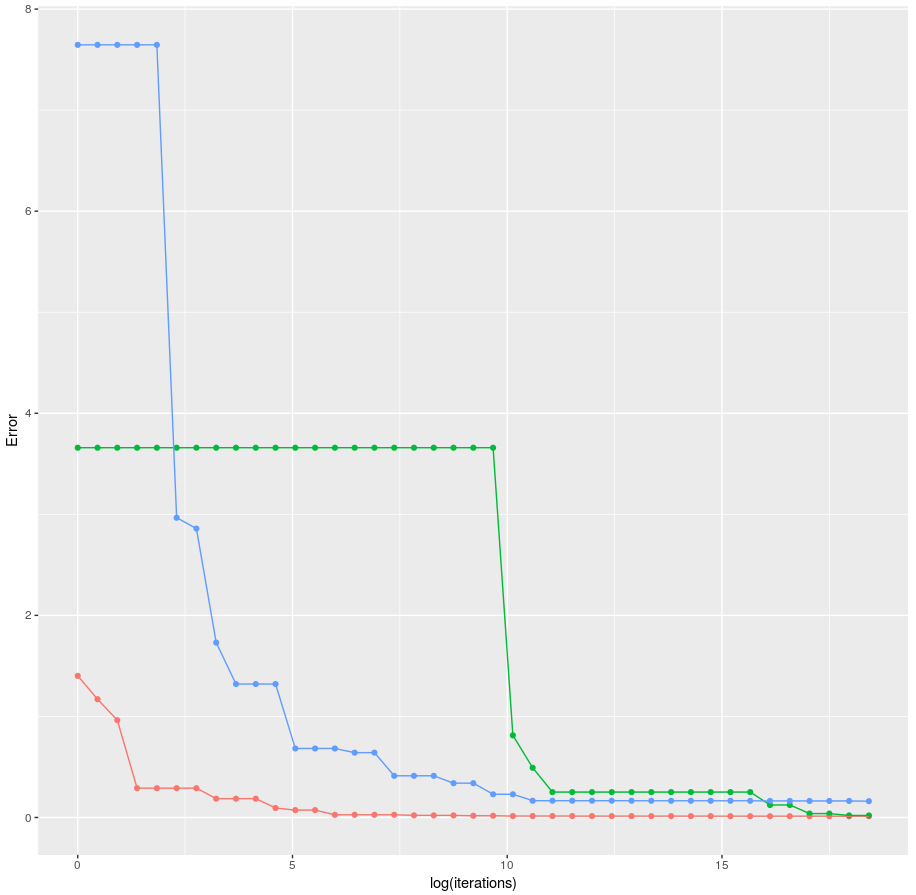
\includegraphics[width = 0.8\columnwidth]{theta}
	\end{center}
	\caption{Comparing different $\hat{\theta}$'s used to estimate $\theta$. The green line is $\hat{\theta_2}$, 
	the blue line is $\hat{\theta_3}$, and the red line is $\theta_1$ \label{fig:theta}}
	\end{figure}
	
	As expected, $\hat{\theta_1}$ gives the lowest error, as we are sampling from the target distribution. We can see that $\hat{\theta_3}$ gives
	a faster convergence than $\hat{\theta_2}$.
	
\section*{Problem 2}
	In this problem, we estimate the number the number of Self-Avoiding Walks in an $(n+1) \times (n+1)$ grid. 
	\subsection{Total number of SAWs for n = 10.}
	We design three different trial probabilities that we use to generate samples. In the first design, we use $$g_1(x) = \prod_{j=1}^m \frac{1}{k_j}$$
	where $m$ is the total length of the path, and $k_j$ is the number of possible choices at the $j$-th step. In the second design, we introduce an option to stop at each step,
	which occurs with probability $\epsilon = 0.1$. In the third design, we keep track of SAWs whose lengths are greater than 50, use these paths to generate $5$ children, and 
	then we average the weights. The log-log plot of the number of SAWs over the number of iterations is shown below:
	
	\begin{figure}[h]
	\begin{center}
		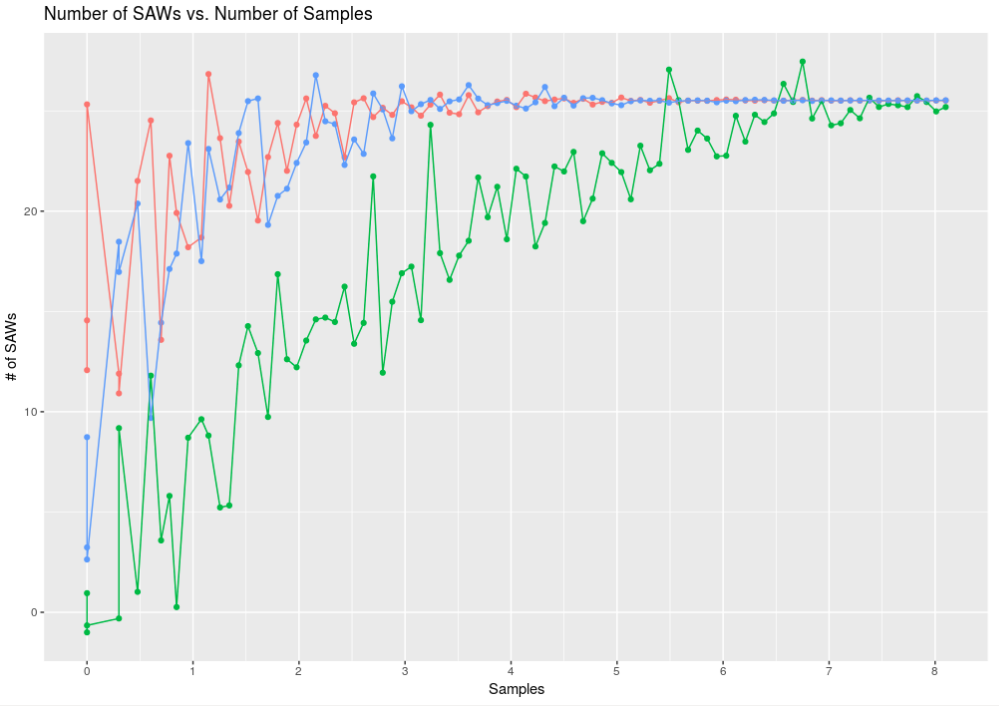
\includegraphics[width = 1.0\columnwidth]{convergence_plot}
	\end{center}
	\caption{SAWs found versus the number of samples. The red line is the 1st design, and the blue line is the 3rd design. The 2nd design exhibits the slowest convergence of the three designs. \label{fig:convergence}}
	\end{figure}
	
	Visually, we see that it takes the 2nd design a considerably longer time for the number of SAWs to converge. The first design estimated $K_1 = 3.33 \times 10^{25}$, 
	the second design estimated $K_2 = 5.45 \times 10^{25}$, and the third design estimated $K = 3.40 \times 10^{25}$. The latter two estimates are a bit short of those
	given in the textbook, but all three of the designs give approximations in the same vicinity. It appears that the third design converges a bit more quickly than the first design.
	
	\subsection{Total number of SAWs that start from (0,0) and end at (n,n).}
	Using the same sampling procedures as before, we can generate approximations of the number of SAWs that end at $(n,n)$. Since the first and third designs exhibit similar behavior,
	we just consider the approximations given by the second and third designs. The second design estimates $K_2 = 5.07 \times 10^{24}$, 
	while the third design estimates $K_3 = 6.13 \times 10^{24}$. The value given in the text is $1.5687 \times 10^{24}$, but our approximations are within reason.
	
	\subsection{Distribution of lengths of the SAWs and Longest SAW}
	
	For part 1, we can plot the histograms, of the lengths of the observed SAWs. Note that when calculating the histograms, we need to incorporate the weights used,
	when generating samples. The distribution for each of the designs is given below from top to bottom in the order of the designed probability.
	\begin{figure}[h]
	\begin{center}
		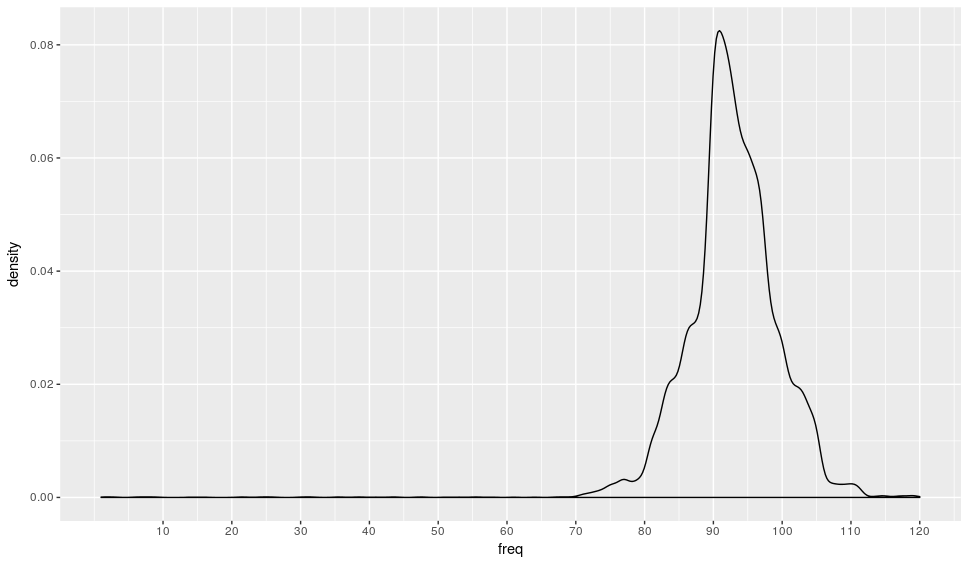
\includegraphics[width = 0.9\columnwidth]{d1}
	\end{center}
	\end{figure}
	
	\vspace{-2mm}	
	
	\begin{figure}[h]
	\begin{center}
		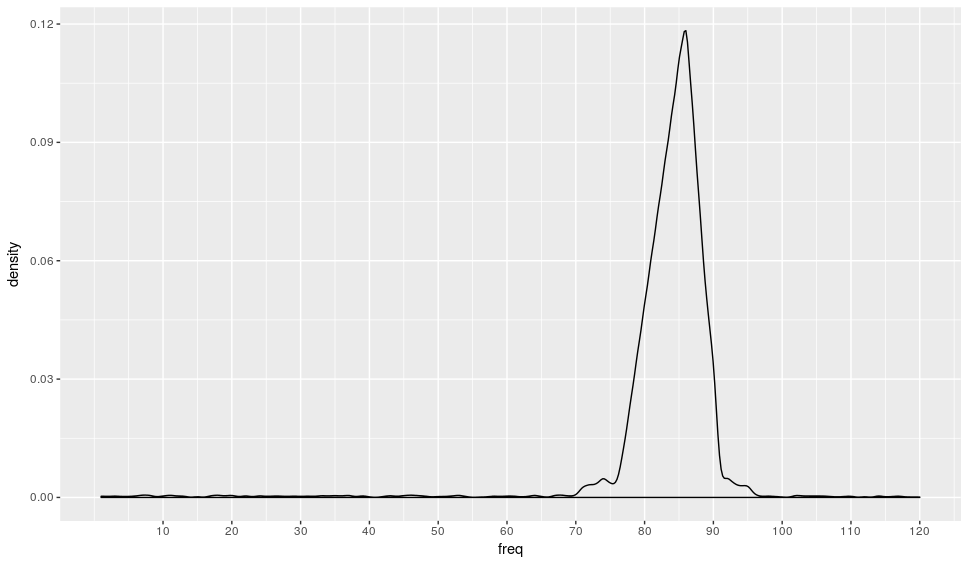
\includegraphics[width = 0.9\columnwidth]{d2}
	\end{center}
	\end{figure}
	
	\vspace{-2mm}
	
	\begin{figure}[h]
	\begin{center}
		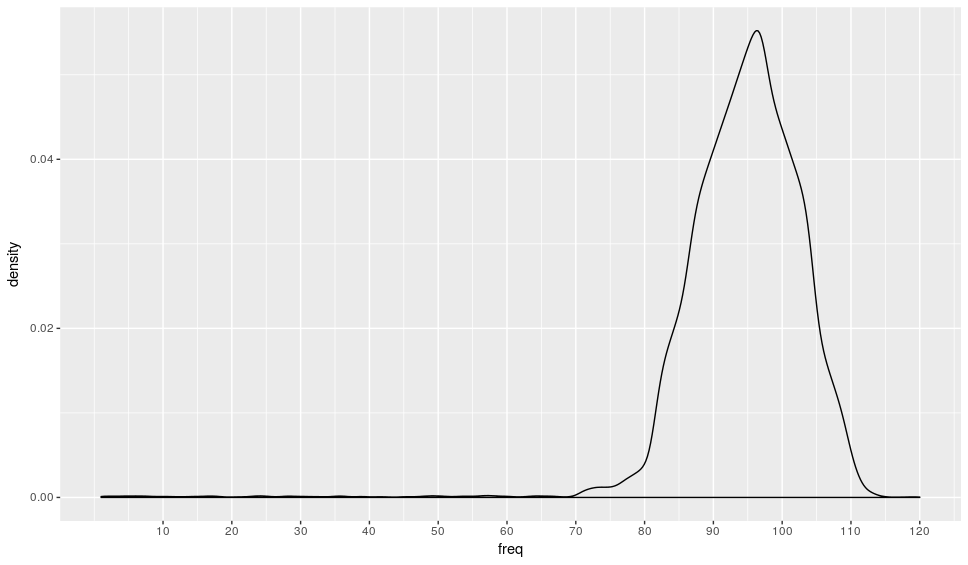
\includegraphics[width = 0.9\columnwidth]{d3}
	\end{center}
	\end{figure}
	
	\vspace{-2mm}
	
	As consistent with the text, the second design favors shorter SAWs, while the third design favors longer walks. When looking for SAWs that end at $(n,n)$,
	the lower tail of the distributions are heavier, since walks that previously contributed to peaks before are now only counted if they end at $(n,n)$. In addition, the peaks are lower since we now only keep track of paths that end up at $(n,n)$. We also visualize the longest SAWs found. Again, we contrast the paths found by design 3 and design 2.
	\vspace{-2mm}
	\begin{figure}[h]
	\begin{center}
		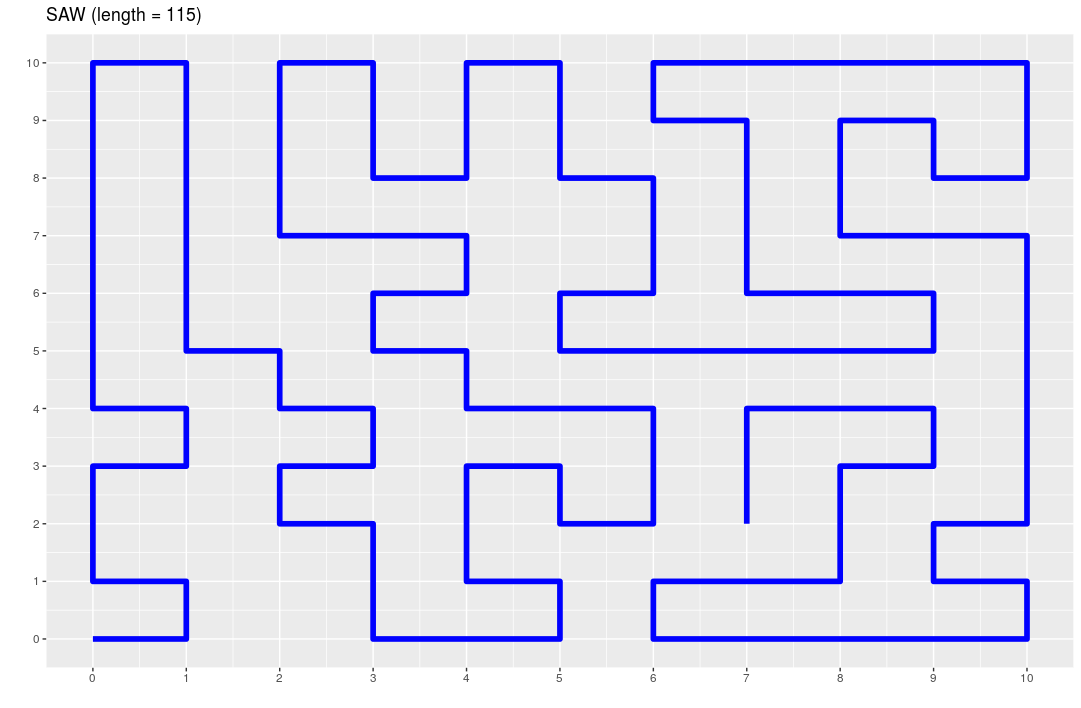
\includegraphics[width = 0.9\columnwidth]{SAW_115}
	\end{center}
	\end{figure}
	
	\vspace{-0.5in}
	
	\begin{figure}[h]
	\begin{center}
		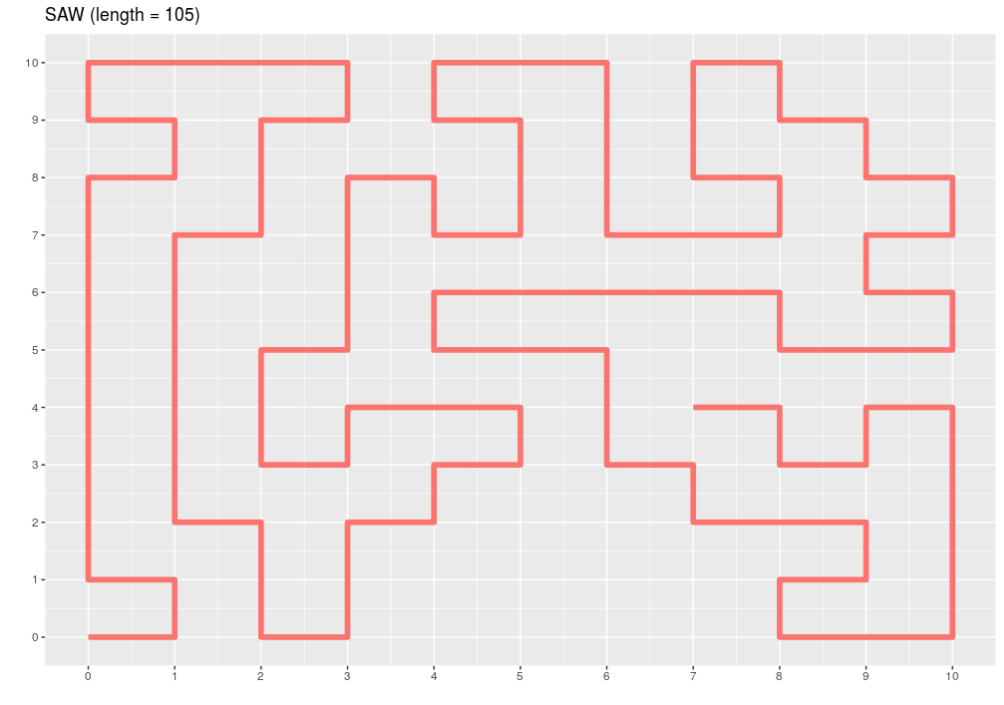
\includegraphics[width = 0.9\columnwidth]{SAW_105}
	\end{center}
	\end{figure}
	
	The third design's longest SAW was 115, as seen in the blue path. The second design's longest SAW was 105, as seen in the red path. 
	This is again what we expect since we included a stopping criteria in the second design. Since we stop more often, the paths tend to be shorter. When searching for
	SAWs that terminate at $(n,n)$, the longest path found by the third design was 112, while the longest path found by the second design was 90. Both paths are shown below, 
	where the blue path is again the SAW from the third design, and the red path is the SAW from the second design. 
	
		\vspace{-2mm}
	
	\begin{figure}[h]
	\begin{center}
		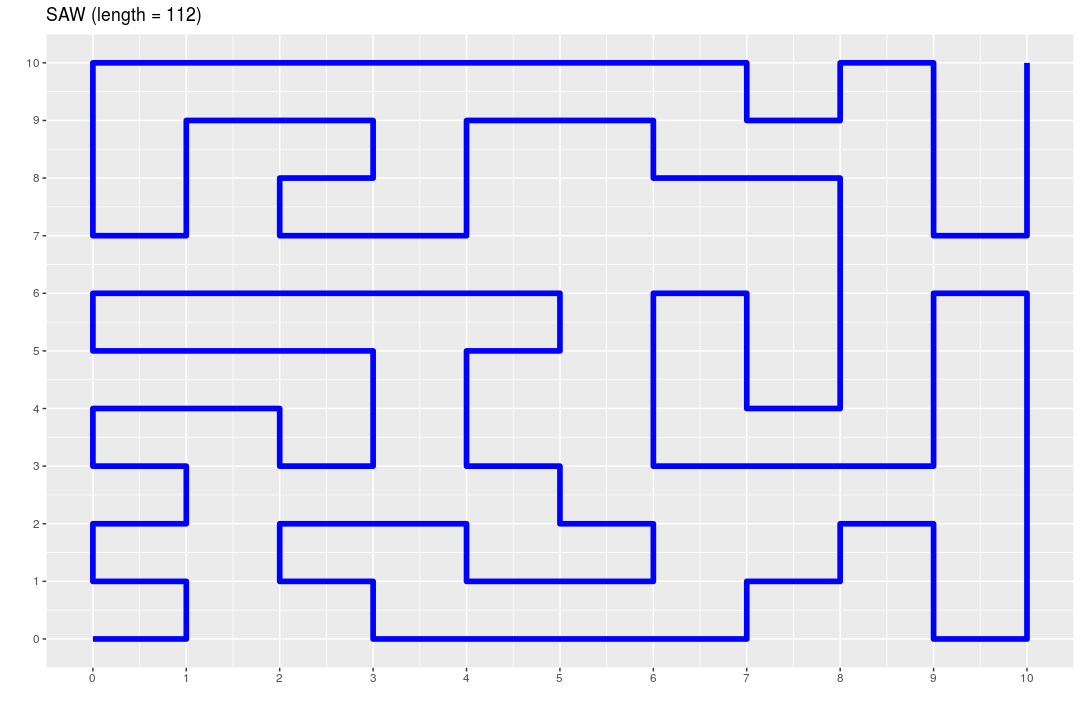
\includegraphics[width = 0.9\columnwidth]{nn_SAW_112}
	\end{center}
	\end{figure}
	
	\begin{figure}[h]
	\begin{center}
		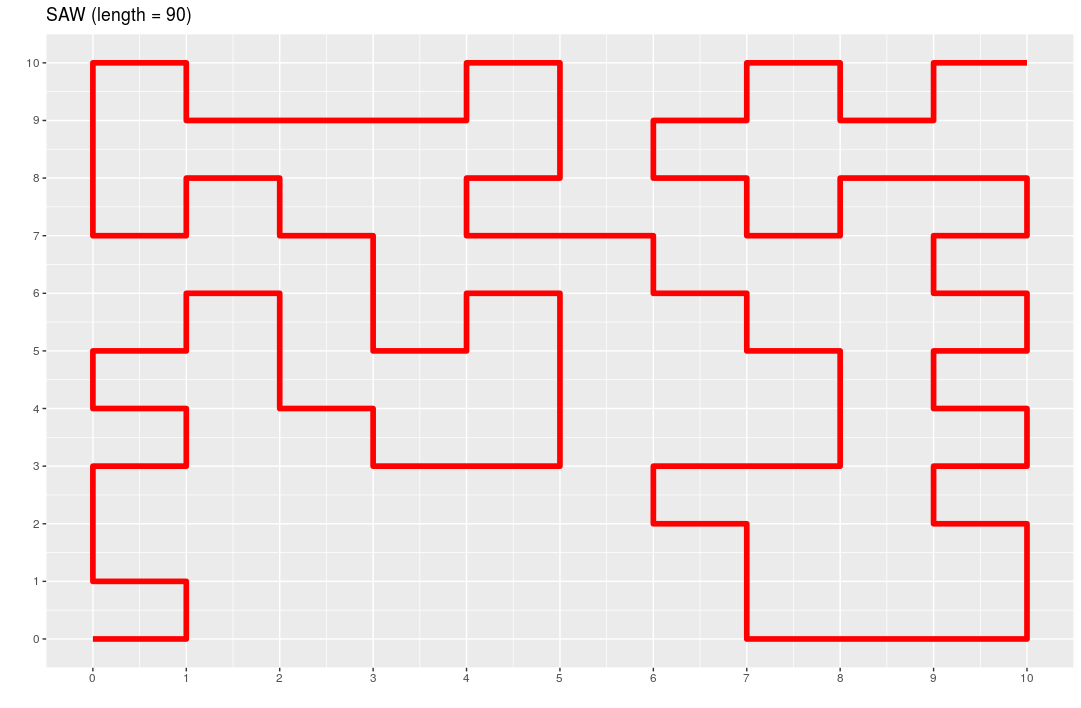
\includegraphics[width = 0.9\columnwidth]{nn_SAW_90}
	\end{center}
	\end{figure}
	
	
	\newpage	
	
	These results continue to match our intuition. Since we only keep track of the paths that terminate at $(n,n)$, we naturally ``lose'' many of the paths for which we
	accounted in part 1. As a result, we are effectively considering a subset of the total SAWs, which consequently gives us SAWs that are shorter in length.
	
	
	

% Your document ends here!
\end{document}